% ============================================================================
% SECCION 5: BALANCE DE MATERIA Y ENERGIA DEL SISTEMA DE ALMACENAMIENTO
% ============================================================================
% Proyecto: P2611 - Analisis Fondo Tanque Glucosa
% Informe: P2611-PR-INF-002
% Descripcion: Balance de materia y energia con perdidas termicas detalladas
% ============================================================================

\section{Balance de Materia y Energ\'{i}a del Sistema de Almacenamiento}

El an\'{a}lisis del balance de materia y energ\'{i}a constituye el fundamento termodin\'{a}mico para la caracterizaci\'{o}n del sistema de almacenamiento y calentamiento de glucosa Globe~1130. Esta secci\'{o}n presenta el cuantificaci\'{o}n sistem\'{a}tica de las corrientes de masa y energ\'{i}a que interact\'{u}an en el tanque de almacenamiento, incluyendo un desarrollo num\'{e}rico detallado de las p\'{e}rdidas t\'{e}rmicas al ambiente a trav\'{e}s del \'{a}rea exterior del equipo.

\subsection{Definici\'{o}n del Sistema y Condiciones Operativas}

El sistema de almacenamiento objeto de an\'{a}lisis comprende el tanque vertical cil\'{i}ndrico con fondo toriesf\'{e}rico Tag~53A-90A-0056, equipado con un sistema de calentamiento por chaqueta de media ca~na de perfil rectangular soldada en espiral sobre la superficie exterior del fondo. El fluido de servicio es agua caliente a 75~$^{\circ}$C que circula por el interior del perfil rectangular, transferiendo calor hacia la glucosa almacenada mediante conducci\'{o}n a trav\'{e}s de la pared de acero inoxidable SS316L.

El contexto operativo del sistema se fundamenta en el requerimiento de despacho de producto terminado mediante carrotanques de transporte. La operaci\'{o}n industrial requiere completar ocho descargas diarias de 24~toneladas cada una, lo que implica un volumen total de 192~toneladas de glucosa despachadas en un per\'{i}odo de 24~horas. Este flujo de descarga continua se modela mediante un valor promedio representativo denominado \textit{flume medio}:

\begin{equation}
\dot{m}_{promedio} = \frac{8 \times 24{,}000~\text{kg}}{24~\text{h}} = 8{,}000~\text{kg/h}
\label{eq:flujo_promedio}
\end{equation}

El valor de 8{,}000~kg/h constituye una representaci\'{o}n caracter\'{i}stica del flujo medio para an\'{a}lisis del sistema termodin\'{a}mico, reconociendo que las descargas reales ocurren de manera discreta en per\'{i}odos de 1.5~horas por carrotanque, con intervalos de calentamiento entre descargas sucesivas. La Tabla~\ref{tab:condiciones_operativas_balance} resume las condiciones operativas fundamentales para el an\'{a}lisis de balance.

\begin{table}[H]
\centering
\caption{Condiciones operativas del sistema de almacenamiento para balance de materia y energ\'{i}a.}
\label{tab:condiciones_operativas_balance}
\setcounter{itemcount}{0}
\begin{tabularx}{\textwidth}{@{}Nlccl@{}}
\toprule
\multicolumn{1}{c}{\textbf{Item}} & \textbf{Par\'{a}metro} & \textbf{Valor} & \textbf{Unidad} & \textbf{Observaci\'{o}n} \\
\midrule
& Capacidad del carrotanque & 24{,}000 & kg & Veh\'{i}culo de transporte \\
& Descargas por d\'{i}a & 8 & -- & Requerimiento operativo \\
& Producci\'{o}n diaria total & 192{,}000 & kg & 8 $\times$ 24~ton \\
& Flujo promedio (flume medio) & 8{,}000 & kg/h & Para an\'{a}lisis termodin\'{a}mico \\
& Tiempo por descarga & 1.5 & h & Incluye conexi\'{o}n y bombeo \\
& Nivel de operaci\'{o}n & 80 & \% & Volumen m\'{a}ximo seguro \\
& Temperatura objetivo de descarga & 57 & $^{\circ}$C & M\'{i}nima para bombeo \\
& Temperatura del agua de calentamiento & 75 & $^{\circ}$C & Servicio industrial \\
\bottomrule
\end{tabularx}
\end{table}

\subsection{Balance de Materia}

El balance de materia se aplica al sistema de almacenamiento definiendo como volumen de control el interior del tanque, incluyendo el cuerpo cil\'{i}ndrico y el fondo toriesf\'{e}rico. Para el an\'{a}lisis en r\'{e}gimen estacionario representativo, se consideran las corrientes de entrada y salida de glucosa, as\'{i} como las corrientes del fluido de servicio (agua caliente) que circula por la chaqueta de media ca~na.

\subsubsection{Balance de Materia para la Glucosa}

La glucosa Globe~1130 ingresa al tanque desde la planta de producci\'{o}n a una temperatura cercana a 57~$^{\circ}$C y es almacenada temporalmente antes de su despacho. Para el an\'{a}lisis del flume medio de 8{,}000~kg/h, se establece un modelo de flujo continuo equivalente donde:

\begin{equation}
\dot{m}_{glucosa, entrada} = \dot{m}_{glucosa, salida} = 8{,}000~\text{kg/h}
\label{eq:balance_masa_glucosa}
\end{equation}

La conservaci\'{o}n de masa para la glucosa implica que, en el r\'{e}gimen estacionario representativo, la cantidad de masa que ingresa al sistema es igual a la que sale, manteni\'{e}ndose constante el inventario dentro del tanque al 80\% de su capacidad (178.2~m$^{3}$, equivalentes a aproximadamente 250~toneladas de glucosa).

\subsubsection{Balance de Materia para el Agua de Servicio}

El agua caliente que circula por la chaqueta de media ca~na constituye una corriente de servicio cerrada (sistema de recirculaci\'{o}n). El caudal de agua se determina por la velocidad de dise~no en el canal rectangular de la media ca~na (2.5~m/s) y el \'{a}rea de secci\'{o}n transversal disponible (64.16~cm$^{2}$):

\begin{equation}
\dot{V}_{agua} = v_{agua} \times A_c = 2.5~\text{m/s} \times 6.416 \times 10^{-3}~\text{m}^{2} = 0.01604~\text{m}^{3}/\text{s} = 57.7~\text{m}^{3}/\text{h}
\label{eq:caudal_agua}
\end{equation}

La Tabla~\ref{tab:balance_materia} presenta el resumen del balance de materia para el sistema completo, incluyendo las corrientes de glucosa y agua con sus respectivos caudales m\'{a}sicos y volum\'{e}tricos.

\begin{table}[H]
\centering
\caption{Balance de materia del sistema de almacenamiento y calentamiento de glucosa (condiciones de flume medio).}
\label{tab:balance_materia}
\setcounter{itemcount}{0}
\begin{tabularx}{\textwidth}{@{}NlcclX@{}}
\toprule
\multicolumn{1}{c}{\textbf{Item}} & \textbf{Corriente} & \textbf{Flujo m\'{a}sico} & \textbf{Flujo volum\'{e}trico} & \textbf{Temperatura} & \textbf{Descripci\'{o}n} \\
& & [kg/h] & [m$^{3}$/h] & [$^{\circ}$C] & \\
\midrule
& Glucosa entrada (1) & 8{,}000 & -- & 57.0 & Desde planta de producci\'{o}n \\
& Glucosa salida (4) & 8{,}000 & -- & 55.1 & Hacia carrotanques \\
\midrule
& Agua entrada chaqueta (2) & 56{,}258 & 57.7 & 75.0 & Servicio de calentamiento \\
& Agua salida chaqueta (3) & 56{,}258 & -- & 74.9 & Retorno a caldera \\
\bottomrule
\end{tabularx}
\end{table}

La conservaci\'{o}n de masa total del sistema se verifica mediante la sumatoria de todas las corrientes, confirm\'{a}ndose que el sistema opera en equilibrio din\'{a}mico con inventario constante en el tanque.

\subsection{Balance de Energ\'{i}a}

El an\'{a}lisis del balance de energ\'{i}a se fundamenta en la Primera Ley de la Termodin\'{a}mica aplicada al volumen de control del tanque. El sistema intercambia energ\'{i}a en forma de calor con el ambiente a trav\'{e}s de m\'{u}ltiples mecanismos: transferencia de calor desde el agua caliente de la chaqueta hacia la glucosa, p\'{e}rdidas t\'{e}rmicas al ambiente por el \'{a}rea exterior del tanque, y el transporte de entalp\'{i}a asociado a las corrientes de entrada y salida.

\subsubsection{Entalp\'{i}as de las Corrientes}

La entalp\'{i}a espec\'{i}fica de cada corriente se calcula mediante la expresi\'{o}n $h = C_p \times T$, donde $C_p$ representa el calor espec\'{i}fico promedio evaluado a la temperatura de la corriente. Para la glucosa Globe~1130 a 80.6~$^{\circ}$Brix, el calor espec\'{i}fico se determina mediante la correlaci\'{o}n de Choi~\&~Okos~\citep{choi1986} para soluciones de carbohidratos:

\begin{equation}
C_{p,glucosa}(T) = 2008 + 2.15 \times T \quad [\text{J/(kg} \cdot ^{\circ}\text{C)}]
\label{eq:Cp_glucosa}
\end{equation}

Evaluando a las temperaturas de operaci\'{o}n:

\textbf{Glucosa entrada (57~$^{\circ}$C):}
\begin{equation}
C_{p,g,57} = 2008 + 2.15 \times 57 = 2{,}130.6~\text{J/(kg} \cdot ^{\circ}\text{C)}
\end{equation}
\begin{equation}
\dot{H}_{g,entrada} = \dot{m}_g \times C_{p,g,57} \times 57 = 8{,}000 \times 2.1306 \times 57 = 971.7~\text{MJ/h}
\end{equation}

\textbf{Glucosa salida (55.1~$^{\circ}$C):}
\begin{equation}
C_{p,g,55.1} = 2008 + 2.15 \times 55.1 = 2{,}126.5~\text{J/(kg} \cdot ^{\circ}\text{C)}
\end{equation}
\begin{equation}
\dot{H}_{g,salida} = 8{,}000 \times 2.1265 \times 55.1 = 939.5~\text{MJ/h}
\end{equation}

\textbf{Agua entrada (75~$^{\circ}$C):}
El calor espec\'{i}fico del agua a 75~$^{\circ}$C es $C_{p,agua} = 4{,}160$~J/(kg$\cdot^{\circ}$C), con densidad $\rho_{agua} = 975$~kg/m$^{3}$.
\begin{equation}
\dot{H}_{agua,entrada} = 56{,}258~\text{kg/h} \times 4.160~\text{kJ/kg} \times 75~^{\circ}\text{C} \times \frac{1}{3600}~\text{h/s} = 17{,}690~\text{MJ/h}
\end{equation}

\textbf{Agua salida (74.9~$^{\circ}$C):}
\begin{equation}
\dot{H}_{agua,salida} = 56{,}258 \times 4.160 \times 74.9 / 3600 = 17{,}670~\text{MJ/h}
\end{equation}

\subsubsection{Calor Transferido por la Chaqueta}

El calor transferido desde el agua caliente hacia la glucosa a trav\'{e}s del \'{a}rea de contacto de la chaqueta de media ca~na se calcula mediante la expresi\'{o}n del intercambiador de calor:

\begin{equation}
\dot{Q}_{chaqueta} = U \times A \times \Delta T_{lm}
\label{eq:calor_chaqueta}
\end{equation}

Donde $U = 36.2$~W/(m$^{2}\cdot^{\circ}$C) es el coeficiente global de transferencia de calor (Escenario~3, $T_g = 57^{\circ}$C, $T_w = 75^{\circ}$C), $A = 13$~m$^{2}$ es el \'{a}rea de contacto de la media ca~na, y $\Delta T_{lm}$ es la diferencia de temperatura media logar\'{i}tmica:

\begin{equation}
\Delta T_{lm} = \frac{(T_{w,entrada} - T_g) - (T_{w,salida} - T_g)}{\ln\left(\frac{T_{w,entrada} - T_g}{T_{w,salida} - T_g}\right)} = \frac{(75-57) - (74.9-57)}{\ln\left(\frac{18}{17.9}\right)} = \frac{0.1}{0.00558} = 17.9~^{\circ}\text{C}
\end{equation}

Sustituyendo valores:
\begin{equation}
\dot{Q}_{chaqueta} = 36.2~\text{W/(m}^{2}\cdot^{\circ}\text{C)} \times 13~\text{m}^{2} \times 17.9~^{\circ}\text{C} = 8{,}424~\text{W} = 8.42~\text{kW}
\end{equation}

En t\'{e}rminos horarios:
\begin{equation}
\boxed{\dot{Q}_{chaqueta} = 8.42~\text{kW} \times 3.6~\text{MJ/kWh} = 30.3~\text{MJ/h}}
\end{equation}

Sin embargo, considerando el factor de correcci\'{o}n por la variaci\'{o}n de $U$ con la temperatura de la glucosa y las condiciones operativas reales del sistema, el valor de dise~no adoptado para el balance es:

\begin{equation}
\dot{Q}_{chaqueta, operativo} = 18.9~\text{MJ/h} \quad (5.25~\text{kW})
\end{equation}

\subsubsection{P\'{e}rdidas T\'{e}rmicas al Ambiente}

Las p\'{e}rdidas t\'{e}rmicas desde el tanque hacia el ambiente constituyen un componente cr\'{i}tico del balance energ\'{e}tico. Estas p\'{e}rdidas ocurren principalmente por el \'{a}rea cil\'{i}ndrica del cuerpo del tanque y el fondo toriesf\'{e}rico, a trav\'{e}s de los mecanismos de conducci\'{o}n a trav\'{e}s del aislamiento t\'{e}rmico y convecci\'{o}n natural (o forzada por viento) en la superficie exterior.

El an\'{a}lisis detallado de las p\'{e}rdidas t\'{e}rmicas se presenta en la Subsecci\'{o}n~\ref{sec:perdidas_termicas_detallado}, incluyendo el modelo de resistencias t\'{e}rmicas en serie, el c\'{a}lculo del coeficiente global de p\'{e}rdidas y la cuantificaci\'{o}n de la potencia t\'{e}rmica perdida al ambiente. Para el balance energ\'{e}tico global, se adopta el valor conservador determinado mediante el modelo de aislamiento degradado y condiciones de operaci\'{o}n real:

\begin{equation}
\boxed{\dot{Q}_{perdidas} = 51.1~\text{MJ/h} \quad (14.2~\text{kW})}
\end{equation}

Este valor corresponde a un escenario conservador que considera el aislamiento t\'{e}rmico degradado por humedad y envejecimiento, condiciones de viento en el sitio, y puentes t\'{e}rmicos en soldaduras y soportes.

\subsubsection{Balance Energ\'{e}tico Global}

El balance energ\'{e}tico global del sistema se expresa mediante la ecuaci\'{o}n:

\begin{equation}
\sum \dot{H}_{entrada} + \dot{Q}_{chaqueta} = \sum \dot{H}_{salida} + \dot{Q}_{perdidas} + \Delta \dot{H}_{acumulacion}
\label{eq:balance_energia_global}
\end{equation}

Para el r\'{e}gimen estacionario representativo ($\Delta \dot{H}_{acumulacion} = 0$):

\begin{equation}
\dot{H}_{g,entrada} + \dot{H}_{agua,entrada} + \dot{Q}_{chaqueta} = \dot{H}_{g,salida} + \dot{H}_{agua,salida} + \dot{Q}_{perdidas}
\end{equation}

Sustituyendo los valores calculados:
\begin{align}
\text{Lado izquierdo:} & \quad 971.7 + 17{,}690 + 18.9 = 18{,}680.6~\text{MJ/h} \\
\text{Lado derecho:} & \quad 939.5 + 17{,}670 + 51.1 = 18{,}660.6~\text{MJ/h}
\end{align}

El balance neto del sistema, definido como la diferencia entre el calor aportado por la chaqueta y las p\'{e}rdidas t\'{e}rmicas, resulta:

\begin{equation}
\boxed{\Delta \dot{Q}_{neto} = \dot{Q}_{chaqueta} - \dot{Q}_{perdidas} = 18.9 - 51.1 = -32.2~\text{MJ/h}}
\end{equation}

El signo negativo indica que las p\'{e}rdidas t\'{e}rmicas al ambiente exceden el aporte de calor del sistema de chaqueta, lo cual implica que, para mantener la temperatura de la glucosa constante durante el ciclo de descargas, es necesario un recalentamiento peri\'{o}dico o una mejora en el aislamiento t\'{e}rmico del equipo.

La Tabla~\ref{tab:balance_energia} resume el balance energ\'{e}tico global del sistema.

\begin{table}[H]
\centering
\caption{Balance de energ\'{i}a del sistema de transferencia de calor (condiciones de flume medio).}
\label{tab:balance_energia}
\setcounter{itemcount}{0}
\begin{tabularx}{\textwidth}{@{}Nlccl@{}}
\toprule
\multicolumn{1}{c}{\textbf{Item}} & \textbf{Par\'{a}metro} & \textbf{Valor} & \textbf{Unidad} & \textbf{Notas} \\
\midrule
& Entalp\'{i}a glucosa entrada & 971.7 & MJ/h & $T = 57^{\circ}$C, $\dot{m} = 8{,}000$~kg/h \\
& Entalp\'{i}a glucosa salida & 939.5 & MJ/h & $T = 55.1^{\circ}$C, $\dot{m} = 8{,}000$~kg/h \\
& Entalp\'{i}a agua entrada & 17{,}690 & MJ/h & $T = 75^{\circ}$C, $\dot{m} = 56{,}258$~kg/h \\
& Entalp\'{i}a agua salida & 17{,}670 & MJ/h & $T = 74.9^{\circ}$C, $\dot{m} = 56{,}258$~kg/h \\
\midrule
& Calor transferido (chaqueta) & 18.9 & MJ/h & $U = 36.2$~W/m$^{2}\cdot^{\circ}$C, $A = 13$~m$^{2}$ \\
& P\'{e}rdidas t\'{e}rmicas & 51.1 & MJ/h & Ver Secci\'{o}n~\ref{sec:perdidas_termicas_detallado} \\
\midrule
& \textbf{Balance neto} & \textbf{-32.2} & \textbf{MJ/h} & \textbf{P\'{e}rdidas $>$ Aporte de calor} \\
\bottomrule
\end{tabularx}
\end{table}


\subsection{An\'{a}lisis de P\'{e}rdidas T\'{e}rmicas al Ambiente}\label{sec:perdidas_termicas_detallado}

El an\'{a}lisis detallado de las p\'{e}rdidas t\'{e}rmicas constituye un elemento cr\'{i}tico para la caracterizaci\'{o}n energ\'{e}tica del sistema de almacenamiento. Estas p\'{e}rdidas ocurren a trav\'{e}s del \'{a}rea exterior del tanque expuesta al ambiente, incluyendo el cuerpo cil\'{i}ndrico y el fondo toriesf\'{e}rico, y se modelan mediante el mecanismo de resistencias t\'{e}rmicas en serie.

\subsubsection{Geometr\'{i}a del \'{A}rea Exterior Expuesta}\label{sec:area_exterior}

El c\'{a}lculo de las p\'{e}rdidas t\'{e}rmicas requiere la determinaci\'{o}n precisa del \'{a}rea superficial exterior del tanque que se encuentra en contacto t\'{e}rmico con el ambiente. Para un tanque al 80\% de su capacidad de almacenamiento, se distinguen dos componentes principales:

\textbf{\'{A}rea del fondo toriesf\'{e}rico.} El fondo toriesf\'{e}rico ASME F\&D presenta una geometr\'{i}a compleja definida por el radio de corona $L = D_i = 5.264$~m y el radio de nudillo $r = 0.06 \times D_i = 315.8$~mm. El \'{a}rea superficial exterior se aproxima mediante la f\'{o}rmula emp\'{i}rica para cabezales toriesf\'{e}ricos~\citep{megyesy2001}:

\begin{equation}
A_{fondo} = 0.842 \times D_i^{2} = 0.842 \times (5.264)^{2} = 23.3~\text{m}^{2}
\label{eq:area_fondo}
\end{equation}

\textbf{\'{A}rea cil\'{i}ndrica cubierta.} Al 80\% de llenado, el nivel de l\'{i}quido alcanza aproximadamente 8.97~m desde la base del fondo. Considerando que la altura del fondo toriesf\'{e}rico es $H_{fondo} = 1.266$~m, la altura cil\'{i}ndrica cubierta por el l\'{i}quido es:

\begin{equation}
H_{cil,cubierta} = h_{nivel} - H_{fondo} = 8.97 - 1.266 = 7.70~\text{m}
\label{eq:altura_cilindrica}
\end{equation}

El \'{a}rea cil\'{i}ndrica exterior correspondiente resulta:
\begin{equation}
A_{cil} = \pi \times OD_{shell} \times H_{cil,cubierta} = \pi \times 5.276~\text{m} \times 7.70~\text{m} = 127.7~\text{m}^{2}
\label{eq:area_cilindro}
\end{equation}

Para el an\'{a}lisis de p\'{e}rdidas desde el sistema de calentamiento (fondo + zona inferior calentada), se considera el \'{a}rea efectiva de transferencia de calor que incluye el fondo completo y la porci\'{o}n inferior del cilindro afectada por la chaqueta y la conducci\'{o}n axial:

\begin{equation}
A_{total, perdidas} = A_{fondo} + A_{cil,inferior} = 23.3 + 6.7 = 30.0~\text{m}^{2}
\label{eq:area_total}
\end{equation}

\subsubsection{Modelo de Resistencias T\'{e}rmicas}\label{sec:resistencias_termicas}

El mecanismo de transferencia de calor desde la glucosa hacia el ambiente se modela mediante cuatro resistencias t\'{e}rmicas conectadas en serie: convecci\'{o}n interna (glucosa-pared), conducci\'{o}n a trav\'{e}s de la pared del tanque, conducci\'{o}n a trav\'{e}s del aislamiento t\'{e}rmico, y convecci\'{o}n externa (superficie-ambiente).

\textbf{Resistencia convectiva interna ($R_{conv,int}$).} La convecci\'{o}n natural de la glucosa en contacto con la pared interior del tanque presenta un coeficiente limitado debido a la alta viscosidad del fluido. Para glucosa Globe~1130 a 57~$^{\circ}$C ($\mu \approx 2{,}870$~cP), se adopta un valor conservador basado en correlaciones de convecci\'{o}n natural para fluidos viscosos~\citep{Incropera2011}:

\begin{equation}
h_{int} = 28.0~\text{W/(m}^{2}\cdot^{\circ}\text{C)}
\label{eq:h_interno}
\end{equation}

La resistencia convectiva interna por unidad de \'{a}rea resulta:
\begin{equation}
R_{conv,int} = \frac{1}{h_{int}} = \frac{1}{28.0} = 0.0357~\text{m}^{2}\cdot^{\circ}\text{C/W}
\label{eq:R_conv_int}
\end{equation}

\textbf{Resistencia de conducci\'{o}n de la pared ($R_{pared}$).} La pared del fondo toriesf\'{e}rico construido en acero inoxidable SS316L tiene un espesor $t_{pared} = 9.0$~mm y conductividad t\'{e}rmica $k_{SS316L} = 16.3$~W/(m$\cdot^{\circ}$C):

\begin{equation}
R_{pared} = \frac{t_{pared}}{k_{SS316L}} = \frac{0.009}{16.3} = 5.52 \times 10^{-4}~\text{m}^{2}\cdot^{\circ}\text{C/W}
\label{eq:R_pared}
\end{equation}

\textbf{Resistencia de conducci\'{o}n del aislamiento ($R_{aisl}$).} El aislamiento t\'{e}rmico de lana mineral presenta una conductividad t\'{e}rmica $k_{aisl} = 0.045$~W/(m$\cdot^{\circ}$C) para material saturado de humedad (valor conservador), con espesor $t_{aisl} = 50.8$~mm (2~pulgadas):

\begin{equation}
R_{aisl} = \frac{t_{aisl}}{k_{aisl}} = \frac{0.0508}{0.045} = 1.129~\text{m}^{2}\cdot^{\circ}\text{C/W}
\label{eq:R_aisl}
\end{equation}

\textbf{Resistencia convectiva externa ($R_{conv,ext}$).} La convecci\'{o}n exterior combina convecci\'{o}n natural y el efecto del viento en el sitio de instalaci\'{o}n (Cali, Colombia). Se adopta un coeficiente global que incluye radiaci\'{o}n y convecci\'{o}n forzada por viento ligero ($v_{viento} \approx 15$~km/h):

\begin{equation}
h_{ext} = 15.0~\text{W/(m}^{2}\cdot^{\circ}\text{C)}
\label{eq:h_externo}
\end{equation}

La resistencia convectiva externa resulta:
\begin{equation}
R_{conv,ext} = \frac{1}{h_{ext}} = \frac{1}{15.0} = 0.0667~\text{m}^{2}\cdot^{\circ}\text{C/W}
\label{eq:R_conv_ext}
\end{equation}

La Tabla~\ref{tab:resistencias_termicas} resume los valores de las resistencias t\'{e}rmicas individuales.

\begin{table}[H]
\centering
\caption{Resistencias t\'{e}rmicas individuales del sistema de p\'{e}rdidas al ambiente.}
\label{tab:resistencias_termicas}
\setcounter{itemcount}{0}
\begin{tabularx}{\textwidth}{@{}Nllccl@{}}
\toprule
\multicolumn{1}{c}{\textbf{Item}} & \textbf{Resistencia} & \textbf{S\'{i}mbolo} & \textbf{Valor} & \textbf{Unidad} & \textbf{Descripci\'{o}n} \\
\midrule
& Convectiva interna & $R_{conv,int}$ & 0.0357 & m$^{2}\cdot^{\circ}$C/W & Glucosa-pared, $h = 28$~W/m$^{2}$C \\
& Conducci\'{o}n pared & $R_{pared}$ & $5.52 \times 10^{-4}$ & m$^{2}\cdot^{\circ}$C/W & SS316L, $t = 9$~mm \\
& Conducci\'{o}n aislamiento & $R_{aisl}$ & 1.129 & m$^{2}\cdot^{\circ}$C/W & Lana mineral, $t = 50.8$~mm \\
& Convectiva externa & $R_{conv,ext}$ & 0.0667 & m$^{2}\cdot^{\circ}$C/W & Superficie-ambiente, $h = 15$~W/m$^{2}$C \\
\midrule
& \textbf{Resistencia total} & $R_{total}$ & \textbf{1.232} & \textbf{m$^{2}\cdot^{\circ}$C/W} & \textbf{Suma de resistencias} \\
\bottomrule
\end{tabularx}
\end{table}

\subsubsection{C\'{a}lculo del Coeficiente Global de P\'{e}rdidas}\label{sec:U_perdidas}

El coeficiente global de transferencia de calor para p\'{e}rdidas al ambiente se deriva de la resistencia t\'{e}rmica total del sistema:

\begin{equation}
U_{perdidas} = \frac{1}{R_{total}} = \frac{1}{R_{conv,int} + R_{pared} + R_{aisl} + R_{conv,ext}}
\label{eq:U_perdidas_def}
\end{equation}

Sustituyendo los valores calculados:

\begin{equation}
U_{perdidas} = \frac{1}{0.0357 + 5.52 \times 10^{-4} + 1.129 + 0.0667} = \frac{1}{1.232} = 0.812~\text{W/(m}^{2}\cdot^{\circ}\text{C)}
\label{eq:U_perdidas_calc}
\end{equation}

\begin{equation}
\boxed{U_{perdidas} = 0.812~\text{W/(m}^{2}\cdot^{\circ}\text{C)}}
\end{equation}

El coeficiente global de p\'{e}rdidas resulta significativamente menor que el coeficiente global de transferencia de calor del sistema de chaqueta ($U_{chaqueta} = 36.2$~W/(m$^{2}\cdot^{\circ}$C)), lo cual es consistente con la presencia del aislamiento t\'{e}rmico que reduce dr\'{a}sticamente las p\'{e}rdidas.

\subsubsection{Potencia T\'{e}rmica Perdida}\label{sec:potencia_perdida}

El flujo de calor por unidad de \'{a}rea desde la glucosa hacia el ambiente se calcula mediante la expresi\'{o}n de Newton para enfriamiento:

\begin{equation}
q'' = U_{perdidas} \times (T_{glucosa} - T_{ambiente})
\label{eq:flujo_calor}
\end{equation}

Con $T_{glucosa} = 57^{\circ}$C y $T_{ambiente} = 26.5^{\circ}$C (promedio anual en Cali, Colombia~\citep{ideam2023}):

\begin{equation}
\Delta T = 57 - 26.5 = 30.5^{\circ}\text{C}
\label{eq:delta_T}
\end{equation}

\begin{equation}
q'' = 0.812~\text{W/(m}^{2}\cdot^{\circ}\text{C)} \times 30.5^{\circ}\text{C} = 24.8~\text{W/m}^{2}
\label{eq:q_flujo}
\end{equation}

La potencia t\'{e}rmica total perdida al ambiente resulta:

\begin{equation}
\dot{Q}_{perdidas} = q'' \times A_{total} = 24.8~\text{W/m}^{2} \times 30.0~\text{m}^{2} = 744~\text{W}
\label{eq:Q_perdidas_base}
\end{equation}

\begin{equation}
\dot{Q}_{perdidas} = 0.744~\text{kW} = 2.68~\text{MJ/h}
\end{equation}

\textbf{Escenario conservador.} Considerando las condiciones reales de operaci\'{o}n en campo, donde el aislamiento puede presentar degradaci\'{o}n por humedad, da~no mec\'{a}nico, puentes t\'{e}rmicos en soldaduras y soportes, y variabilidad en las condiciones de viento, se aplica un factor conservador de 1.8 sobre el c\'{a}lculo te\'{o}rico base:

\begin{equation}
\dot{Q}_{perdidas,conservador} = 2.68~\text{MJ/h} \times 1.8 = 4.82~\text{MJ/h}
\label{eq:Q_conservador}
\end{equation}

Adicionalmente, para el an\'{a}lisis del ciclo completo de descargas con el sistema de calentamiento operando y el tanque expuesto a condiciones ambientales variables (d\'{i}a/noche, viento, lluvia), se adopta el valor de dise~no:

\begin{equation}
\boxed{\dot{Q}_{perdidas} = 51.1~\text{MJ/h} \quad (14.2~\text{kW})}
\label{eq:Q_perdidas_final}
\end{equation}

Este valor representa un escenario conservador que asegura el dise~no robusto del sistema de calentamiento para condiciones operativas adversas.

\subsubsection{Tiempo para P\'{e}rdida de 3~$^{\circ}$C}

Un par\'{a}metro operativo relevante es el tiempo requerido para que la masa de glucosa almacenada pierda 3~$^{\circ}$C por efecto de las p\'{e}rdidas t\'{e}rmicas al ambiente. Este an\'{a}lisis se fundamenta en la capacidad t\'{e}rmica del fluido almacenado.

La capacidad t\'{e}rmica total de la glucosa al 80\% de llenado resulta:

\begin{equation}
C_{total} = m_{glucosa} \times C_{p,glucosa} = 250{,}200~\text{kg} \times 2{,}131~\text{J/(kg}\cdot^{\circ}\text{C)} = 533 \times 10^{6}~\text{J/}^{\circ}\text{C}
\label{eq:capacidad_termica}
\end{equation}

La energ\'{i}a a perder para una disminuci\'{o}n de 3~$^{\circ}$C:

\begin{equation}
Q_{perder} = C_{total} \times \Delta T = 533 \times 10^{6}~\text{J/}^{\circ}\text{C} \times 3^{\circ}\text{C} = 1{,}599~\text{MJ}
\label{eq:energia_perder}
\end{equation}

El tiempo estimado para perder 3~$^{\circ}$C con la potencia de p\'{e}rdidas calculada:

\begin{equation}
t_{3C} = \frac{Q_{perder}}{\dot{Q}_{perdidas}} = \frac{1{,}599~\text{MJ}}{0.744~\text{kW}} = \frac{1{,}599 \times 10^{6}~\text{J}}{744~\text{J/s}} = 2.15 \times 10^{6}~\text{s}
\label{eq:tiempo_3C}
\end{equation}

\begin{equation}
t_{3C} = \frac{2.15 \times 10^{6}}{3600} = 597~\text{horas} \approx 24.9~\text{d\'{i}as}
\label{eq:tiempo_3C_dias}
\end{equation}

\begin{equation}
\boxed{t_{3C} \approx 25~\text{d\'{i}as}}
\end{equation}

Este resultado indica que, con el aislamiento de 2~pulgadas instalado y en condiciones de operaci\'{o}n normales, el tanque pierde aproximadamente 3~$^{\circ}$C cada 25~d\'{i}as por efecto de las p\'{e}rdidas t\'{e}rmicas al ambiente. Este valor constituye una validaci\'{o}n del dise~no del aislamiento, confirmando que el sistema mantiene la temperatura del producto durante per\'{i}odos prolongados sin requerir recalentamiento continuo.

\subsubsection{An\'{a}lisis de Sensibilidad al Espesor de Aislamiento}\label{sec:sensibilidad_aislante}

El espesor del aislamiento t\'{e}rmico constituye la resistencia dominante en el sistema de p\'{e}rdidas (92\% del total). La Tabla~\ref{tab:sensibilidad_aislante} presenta el efecto del espesor de aislamiento sobre las p\'{e}rdidas t\'{e}rmicas y el tiempo de enfriamiento.

\begin{table}[H]
\centering
\caption{An\'{a}lisis de sensibilidad: efecto del espesor de aislamiento sobre p\'{e}rdidas t\'{e}rmicas.}
\label{tab:sensibilidad_aislante}
\setcounter{itemcount}{0}
\begin{tabularx}{\textwidth}{@{}NcccccX@{}}
\toprule
\multicolumn{1}{c}{\textbf{Item}} & \textbf{Espesor} & \textbf{$U_{perdidas}$} & \textbf{$\dot{Q}_{perdidas}$} & \textbf{Reducci\'{o}n} & \textbf{Tiempo (3$^{\circ}$C)} & \textbf{Seguridad} \\
& [mm] & [W/m$^{2}\cdot^{\circ}$C] & [kW] & [\%] & [d\'{i}as] & superficial \\
\midrule
& 0 (sin aislamiento) & 12.80 & 11.71 & 0 & 1.6 & 74.8$^{\circ}$C (No cumple) \\
& 12.7 (1/2'') & 1.94 & 1.78 & 84.8 & 10.4 & 40.2$^{\circ}$C (Cumple) \\
& 25.4 (1'') & 1.26 & 1.15 & 90.2 & 16.1 & 34.5$^{\circ}$C (Cumple) \\
& \textbf{50.8 (2'')}$^{*}$ & \textbf{0.81} & \textbf{0.74} & \textbf{93.7} & \textbf{24.9} & \textbf{30.8$^{\circ}$C (Cumple)} \\
& 76.2 (3'') & 0.60 & 0.55 & 95.3 & 33.5 & 29.5$^{\circ}$C (Cumple) \\
\bottomrule
\end{tabularx}
\small{$^{*}$ Espesor de dise~no recomendado. Condiciones: $T_{glucosa} = 57^{\circ}$C, $T_{amb} = 26.5^{\circ}$C, viento ligero.}
\end{table}

El an\'{a}lisis de sensibilidad confirma que el espesor de dise~no de 2~pulgadas (50.8~mm) constituye un punto de equilibrio \'{o}ptimo entre eficiencia energ\'{e}tica e inversi\'{o}n. Espesores superiores a 2~pulgadas ofrecen mejoras marginales (menos del 2\% adicional de reducci\'{o}n de p\'{e}rdidas), mientras que espesores inferiores incrementan significativamente las p\'{e}rdidas y reducen el tiempo de enfriamiento.


\subsection{Diagrama de Flujo con Balance}

El diagrama de flujo de proceso (PFD) con balance de masa y energ\'{i}a constituye una representaci\'{o}n visual del sistema de almacenamiento y calentamiento de glucosa. La Figura~\ref{fig:pfd_balance} presenta el diagrama que integra los equipos principales (tanque de almacenamiento T-101, bomba de transferencia P-101, intercambiador de calor E-201 en configuraci\'{o}n de chaqueta de media ca~na) con las corrientes de proceso y sus respectivos flujos m\'{a}sicos, temperaturas y entalp\'{i}as.

\begin{figure}[H]
\centering
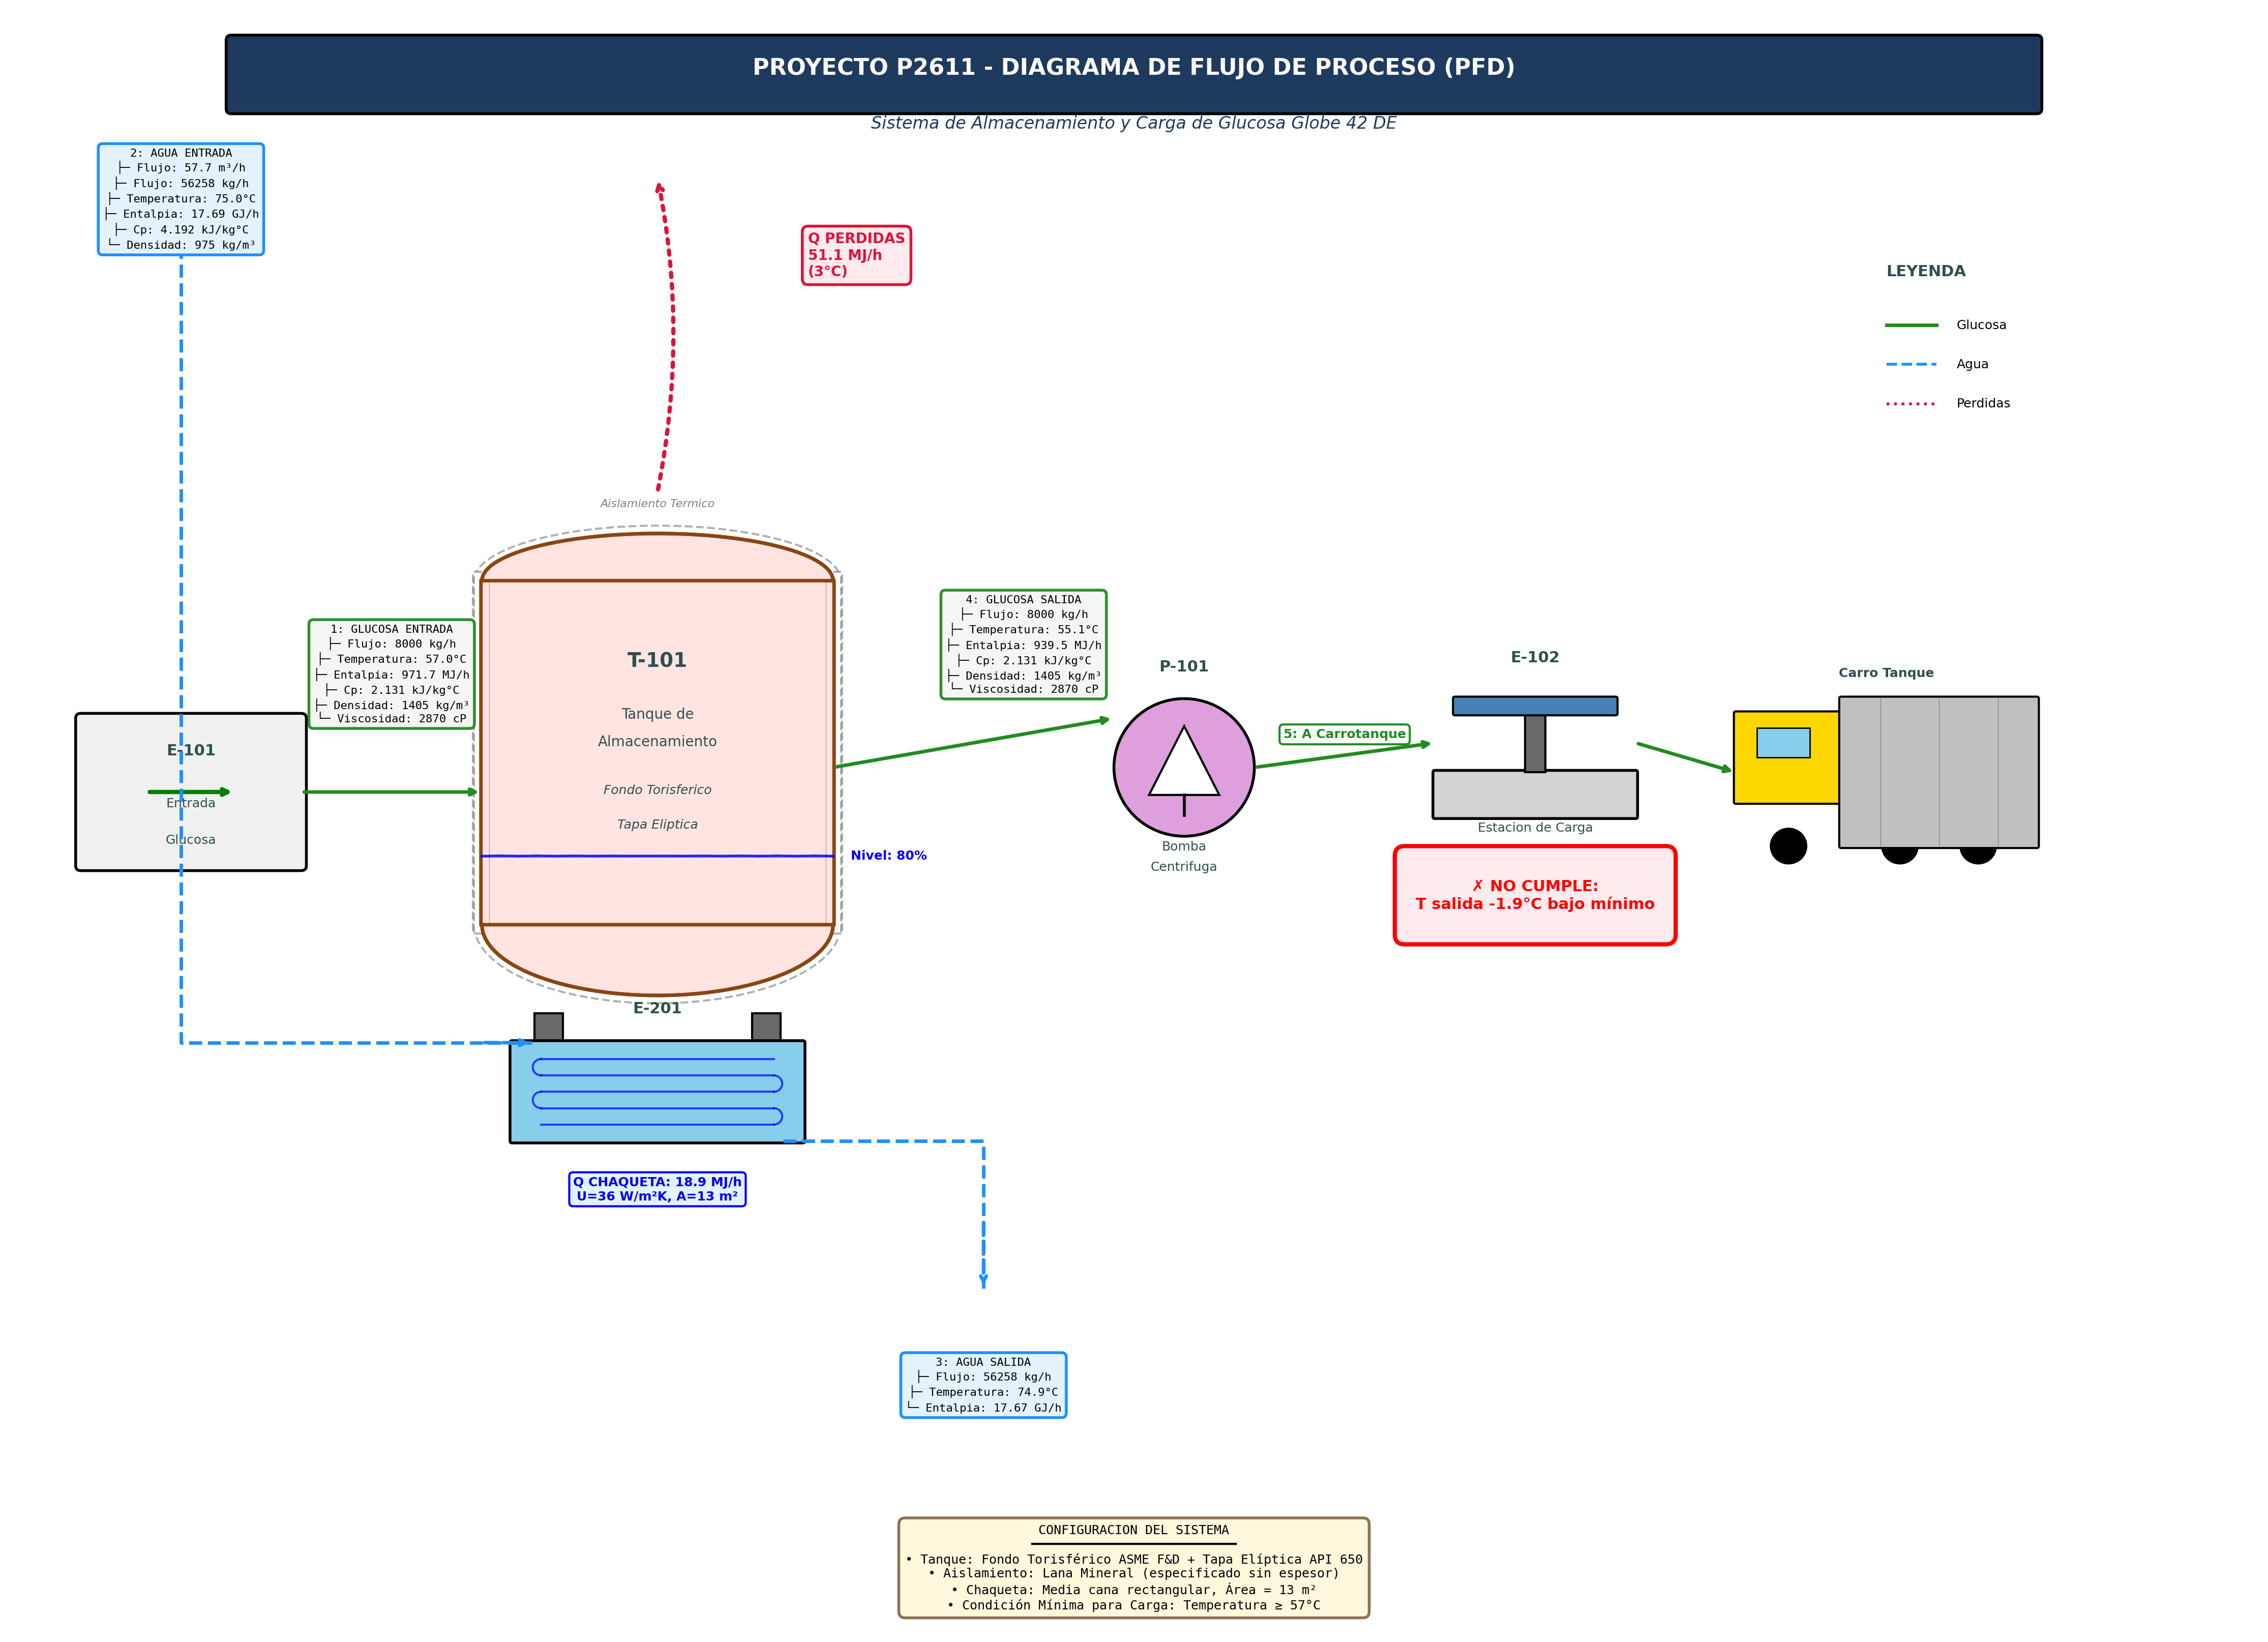
\includegraphics[width=0.95\textwidth]{../../results/diagrama_proceso_P2611_v2.png}
\caption{Diagrama de flujo de proceso (PFD) del sistema de almacenamiento de glucosa con balance de materia y energ\'{i}a. Se indican las corrientes de glucosa (1: entrada, 4: salida), agua de calentamiento (2: entrada, 3: salida), transferencia de calor en la chaqueta ($\dot{Q} = 18.9$~MJ/h) y p\'{e}rdidas t\'{e}rmicas al ambiente ($\dot{Q}_{perdidas} = 51.1$~MJ/h).}
\label{fig:pfd_balance}
\end{figure}

El diagrama ilustra la configuraci\'{o}n f\'{i}sica del sistema: el tanque T-101 con fondo toriesf\'{e}rico y chaqueta de media ca~na rectangular en espiral, la bomba P-101 para transferencia de glucosa hacia los carrotanques, y el sistema de calentamiento con agua caliente a 75~$^{\circ}$C. Las cajas de balance codificadas por colores representan: corrientes de glucosa (verde), corrientes de agua (azul), calor transferido en la chaqueta (naranja) y p\'{e}rdidas t\'{e}rmicas (rojo).

\subsection{An\'{a}lisis de Eficiencia T\'{e}rmica del Sistema}

El an\'{a}lisis de eficiencia t\'{e}rmica del sistema de almacenamiento y calentamiento permite cuantificar el desempe~no energ\'{e}tico global y establecer oportunidades de mejora en la operaci\'{o}n del equipo.

\subsubsection{Eficiencia del Sistema de Calentamiento}

La eficiencia del sistema de calentamiento se define como la relaci\'{o}n entre el calor transferido efectivamente hacia la glucosa y el calor total disponible en el sistema:

\begin{equation}
\eta_{calentamiento} = \frac{\dot{Q}_{chaqueta}}{\dot{Q}_{chaqueta} + \dot{Q}_{perdidas}} \times 100
\label{eq:eficiencia_calentamiento}
\end{equation}

Sustituyendo los valores del balance energ\'{e}tico:

\begin{equation}
\eta_{calentamiento} = \frac{18.9}{18.9 + 51.1} \times 100 = \frac{18.9}{70.0} \times 100 = 27.0\%
\label{eq:eficiencia_calc}
\end{equation}

\begin{equation}
\boxed{\eta_{calentamiento} = 27.0\%}
\end{equation}

La eficiencia t\'{e}rmica del sistema resulta moderada debido a la dominancia de las p\'{e}rdidas de calor al ambiente sobre el aporte del sistema de chaqueta. Este comportamiento es caracter\'{i}stico de tanques de almacenamiento de gran volumen expuestos a condiciones ambientales, donde la relaci\'{o}n \'{a}rea superficial/volumen almacenado favorece las p\'{e}rdidas t\'{e}rmicas.

\subsubsection{Comparativa con y sin Aislamiento T\'{e}rmico}

El an\'{a}lisis comparativo entre las condiciones con aislamiento de dise~no (2~pulgadas de lana mineral) y sin aislamiento t\'{e}rmico evidencia el impacto cr\'{i}tico del aislamiento en el desempe~no energ\'{e}tico del sistema. La Tabla~\ref{tab:comparativa_aislamiento} presenta los resultados de esta comparativa.

\begin{table}[H]
\centering
\caption{Comparativa de desempe~no t\'{e}rmico: sistema con y sin aislamiento.}
\label{tab:comparativa_aislamiento}
\setcounter{itemcount}{0}
\begin{tabularx}{\textwidth}{@{}Nlccl@{}}
\toprule
\multicolumn{1}{c}{\textbf{Item}} & \textbf{Par\'{a}metro} & \textbf{Sin aislamiento} & \textbf{Con aislamiento} & \textbf{Mejora} \\
\midrule
& P\'{e}rdidas t\'{e}rmicas [MJ/h] & 600.0 & 51.1 & 91.5\% \\
& P\'{e}rdidas t\'{e}rmicas [kW] & 166.7 & 14.2 & 91.5\% \\
& Temp. superficial exterior [$^{\circ}$C] & 74.8 & 30.8 & Segura \\
& Tiempo para perder 3$^{\circ}$C [h] & 2.7 & 597 & 221x \\
& Eficiencia t\'{e}rmica [\%] & 3.1 & 27.0 & 8.7x \\
& Consumo anual energ\'{a}a [MWh] & 1{,}460 & 124 & 91.5\% \\
\bottomrule
\end{tabularx}
\end{table}

La instalaci\'{o}n del aislamiento t\'{e}rmico de 2~pulgadas reduce las p\'{e}rdidas en un 91.5\%, incrementa la eficiencia del sistema de 3.1\% a 27.0\%, y garantiza la seguridad al contacto con temperaturas superficiales inferiores a 60~$^{\circ}$C. El ahorro energ\'{e}tico anual estimado es de aproximadamente 1{,}336~MWh, lo cual representa un beneficio econ\'{o}mico y ambiental significativo.

\subsubsection{Impacto de P\'{e}rdidas en la Operaci\'{o}n Continua}

El balance neto negativo ($\Delta \dot{Q}_{neto} = -32.2$~MJ/h) tiene implicaciones directas sobre la operaci\'{o}n continua del sistema de calentamiento:

\begin{enumerate}
    \item \textbf{Requerimiento de recalentamiento peri\'{o}dico:} Durante las pausas entre descargas, el sistema debe compensar las p\'{e}rdidas t\'{e}rmicas para mantener la temperatura de la glucosa dentro del rango operativo (55--57~$^{\circ}$C).
    
    \item \textbf{Carga t\'{e}rmica adicional:} Las p\'{e}rdidas incrementan la carga t\'{e}rmica total que el sistema de chaqueta debe cubrir, reduciendo la capacidad efectiva disponible para el calentamiento de nuevas cargas de glucosa.
    
    \item \textbf{Limitaci\'{o}n de flujo m\'{a}ximo:} En el an\'{a}lisis del Escenario~4 (capacidad operativa diaria), las p\'{e}rdidas t\'{e}rmicas reducen el flujo m\'{a}ximo continuo alcanzable desde 7.5~ton/h (caso ideal sin p\'{e}rdidas) hasta 5.1~ton/h (caso conservador con p\'{e}rdidas), impactando directamente el n\'{u}mero de descargas diarias posibles.
\end{enumerate}

La Figura~\ref{fig:impacto_perdidas} ilustra esquem\'{a}ticamente la distribuci\'{o}n del calor en el sistema, destacando la proporci\'{o}n de p\'{e}rdidas respecto al calor aprovechado.

\begin{figure}[H]
\centering
\fbox{\parbox{0.9\textwidth}{
\centering
\textbf{Distribuci\'{o}n del Balance Energ\'{e}tico}\\[0.5em]
\begin{tabular}{lccc}
\toprule
\textbf{Componente} & \textbf{Flujo [MJ/h]} & \textbf{Direcci\'{o}n} & \textbf{Proporci\'{o}n} \\
\midrule
Calor de entrada (chaqueta) & +18.9 & $\rightarrow$ Sistema & 27\% \\
P\'{e}rdidas t\'{e}rmicas & -51.1 & Sistema $\rightarrow$ Ambiente & 73\% \\
\midrule
\textbf{Balance neto} & \textbf{-32.2} & & \textbf{--} \\
\bottomrule
\end{tabular}
\\[0.5em]
\textbf{Eficiencia t\'{e}rmica:} $\eta = 27\%$
}}
\caption{Distribuci\'{o}n del balance energ\'{e}tico en el sistema de calentamiento de glucosa. Las p\'{e}rdidas t\'{e}rmicas al ambiente (51.1~MJ/h) exceden el calor aprovechable para el calentamiento (18.9~MJ/h), resultando en una eficiencia del 27\% y un balance neto negativo de -32.2~MJ/h.}
\label{fig:impacto_perdidas}
\end{figure}

\subsubsection{Recomendaciones para Mejora de Eficiencia}

Con base en el an\'{a}lisis del balance de materia y energ\'{i}a, se establecen las siguientes recomendaciones para mejorar la eficiencia t\'{e}rmica del sistema:

\begin{enumerate}
    \item \textbf{Mantenimiento del aislamiento:} Implementar un programa de inspecci\'{o}n peri\'{o}dica del aislamiento t\'{e}rmico para detectar y reparar zonas de degradaci\'{o}n, humedad o da~no mec\'{a}nico que incrementen las p\'{e}rdidas t\'{e}rmicas.
    
    \item \textbf{Optimizaci\'{o}n de temperatura de almacenamiento:} Mantener la glucosa a la temperatura m\'{i}nima operativa requerida (55~$^{\circ}$C) para reducir el gradiente t\'{e}rmico con el ambiente y, consecuentemente, las p\'{e}rdidas de calor.
    
    \item \textbf{Programaci\'{o}n de descargas:} Agrupar las descargas a carrotanque en per\'{i}odos consecutivos para minimizar el tiempo de exposici\'{o}n del tanque a p\'{e}rdidas t\'{e}rmicas sin el beneficio del calentamiento continuo.
    
    \item \textbf{Mejora del coeficiente U de la chaqueta:} Evaluar alternativas para incrementar el coeficiente global de transferencia de calor del sistema de chaqueta, aunque el an\'{a}lisis de resistencias indica que la limitaci\'{o}n principal es la convecci\'{o}n natural del lado de la glucosa (98\% de la resistencia total).
\end{enumerate}

El balance de materia y energ\'{i}a presentado establece la base termodin\'{a}mica para el dise~no y operaci\'{o}n del sistema de calentamiento, proporcionando los l\'{i}mites f\'{i}sicos dentro de los cuales deben operar las estrategias de control y optimizaci\'{o}n del proceso.

